%\documentclass[a4paper,10pt]{article}
%\documentclass{beamer}
% \documentclass[a4,notes]{seminar}
\documentclass[
	handout,
	notheorems,noamsthm]{beamer}

% Beamer already defines lemma, definition, etc. -> use notheorems
% ftp://ftp.mpi-sb.mpg.de/pub/tex/mirror/ftp.dante.de/pub/tex/macros/latex/contrib/beamer/doc/beameruserguide.pdf
% http://www2.informatik.hu-berlin.de/~mischulz/beamer.html

\usepackage[utf8x]{inputenc}
\usepackage{palatino} %Schriftart

%\usepackage{titlesec}
%\usepackage[fleqn]{amsmath}
\usepackage{amsthm}
\usepackage{amstext}
\usepackage{amssymb}
\usepackage{mathtools}
\usepackage{xparse}
\usepackage{url}
\usepackage{cleveref}
\usepackage{mdframed}
\usepackage{tikz}


%!TEX root =  index.tex

% some useful stuff:
% http://www.automata.rwth-aachen.de/material/skripte/latex/latex.pdf
% http://en.wikibooks.org/wiki/LaTeX/Mathematics
% http://en.wikibooks.org/wiki/LaTeX/Advanced_Mathematics
% http://en.wikibooks.org/wiki/LaTeX/Theorems

\newtheorem{thm}{Theorem}[section]
\newtheorem{lem}[thm]{Lemma}

\theoremstyle{definition}\newtheorem{mydef}{Definition}[section]
\theoremstyle{plain}\newtheorem{lemma}{Lemma}[section]
\theoremstyle{definition}\newtheorem{algo}{Algorithm}[section]

\newcommand{\K}{\mathcal{K}}
\newcommand{\Reg}{\text{Reg}}
\newcommand{\Lang}{\mathcal{L}}
\newcommand{\A}{\mathcal{A}}
\newcommand{\T}{\mathcal{T}}
\newcommand{\F}{\mathcal{F}}
\newcommand{\Q}{\mathbb{Q}}
\newcommand{\R}{\mathbb{R}}
\newcommand{\N}{\mathbb{N}}
\newcommand{\B}{\mathbb{B}}
\newcommand{\Power}{\mathcal{P}}

\newcommand{\mathtext}[1]{\textup{\textrm{#1}}}
\newcommand{\PT}{\mathtext{PT}}
\newcommand{\LT}{\mathtext{LT}}

% got some help here: http://tex.stackexchange.com/questions/13554/define-something-like-lim-but-for-another-name

\newcommand{\ext}{\operatorname{ext}}
\newcommand{\Inf}{\operatorname{Inf}}
\newcommand{\BC}{\operatorname{BC}}
\newcommand{\dext}{\operatorname{\overline{ext}}}
\newcommand{\dlim}{\operatorname{\overline{lim}}}
\newcommand{\Kleene}{\operatorname{\widehat{Kleene}}}
\newcommand{\limClosure}{\operatorname{\widehat{lim}}}
\newcommand{\Occ}{\operatorname{Occ}}
\newcommand{\existsinf}{\exists^\omega}
\newcommand{\overx}{\overset{\times}}
%\newcommand{\overx}{\stackrel{\times}}
\newcommand{\Ax}{\overx{\A}}
\newcommand{\Langreg}{\Lang^*(\text{reg})}
\newcommand{\LangOreg}{\Lang^\omega(\text{reg})}

\newcommand{\defword}[1]{{\bf #1}}

% inspired by http://ftp.fernuni-hagen.de/ftp-dir/pub/mirrors/www.ctan.org/macros/latex/contrib/braket/braket.sty
\def\mid@vertical{\mskip1mu\vrule\mskip1mu}
\def\midvert{\egroup\;\mid@vertical\;\bgroup}
\NewDocumentCommand\Set{mg}{%
    \IfNoValueTF{#2}{%
        \ensuremath{\left\{ #1 \right\}}%
    }{%
        \ensuremath{\left\{ {#1} \;\mid@vertical\; {#2} \right\}}%
    }%
}

%\newcommand{\SetS}[1]{\bigl\{ #1 \bigr\}}
%\newcommand{\SetC}[2]{\bigl\{ #1 \bigm| #2 \bigr\}}
%\DeclarePairedDelimiterX\SetC[2]{\lbrace}{\rbrace}{ #1 \,\delimsize|\, #2 }

%\newcommand{\abs}[1]{\mathopen| #1 \mathclose|}
%\newcommand{\Abs}[1]{\left| #1 \right|}
\newcommand{\abs}[1]{\left| #1 \right|}

% http://de.wikibooks.org/wiki/LaTeX-W%C3%B6rterbuch:_today
\def\monthgerman{\ifcase\month \or
  Januar\or Februar\or M\"arz\or April\or Mai\or Juni\or
  Juli\or August\or September\or Oktober\or November\or Dezember\fi}
\def\todaygerman{\number\day.~\monthgerman\space\number\year}


% for PDF
\subject{a structure theory for Omega-languages}
%\keywords{Omega, language}

\title[Kurzform]{Language Operations and a Structure Theory of $\omega$-Languages}
%\subtitle[Kurzform]{Untertitel}
%\author[A. Zeyer]{Albert Zeyer}
%\institute[i7 RWTH]{Lehrstuhl für Informatik 7}
\date{\today}
%\logo{\pgfimage[width=2cm,height=2cm]{hulogo}}
%\titlegraphic{\includegraphics[width=2cm,height=2cm]{hulogo}}

 
\begin{document}

\frame{\titlepage}

%\frame{
%	\frametitle{Inhaltsverzeichnis}
%	\tableofcontents
%	[pausesections]
%}

\begin{frame}[<+->]{Introduction: $\Power(\Sigma^*) \rightarrow \Power(\Sigma^*)$}
We have the common $\Power(\Sigma^*) \rightarrow \Power(\Sigma^*)$ language operators:

\begin{enumerate}
\item $\ext(L) := \Set{\alpha \in \Sigma^\omega}{ \exists n \colon \alpha[0,n] \in L} = L \cdot \Sigma^\omega$
\item $\dext(L) := \Set{\alpha \in \Sigma^\omega}{ \forall n \colon \alpha[0,n] \in L}$
\item $\lim(L) := \Set{ \alpha \in \Sigma^\omega }{ \forall N \colon \exists n > N \colon \alpha[0,n] \in L } = \Set{ \alpha \in \Sigma^\omega }{ \exists^\omega n \colon \alpha[0,n] \in L }$
\item $\dlim(L) := \Set{ \alpha \in \Sigma^\omega }{ \exists N \colon \forall n > N \colon \alpha[0,n] \in L }$
%\item Kleene-Closure of $\K$: $\bigcup_{i=1}^n U_i \cdot V_i^\omega$, $U_i, V_i \in \K$
\end{enumerate}
\end{frame}

\begin{frame}[<+->]{Introduction: $\Power(\Power(\Sigma^*)) \rightarrow \Power(\Power(\Sigma^*))$}
From these, define language class operators:

\begin{enumerate}
\item $\ext(\Lang) := \Set{\lim L}{L \in \Lang}$
\item $\dext(\Lang) := \Set{\dext L}{L \in \Lang}$
\item $\lim(\Lang) := \Set{\lim L}{L \in \Lang}$
\item $\dlim(\Lang) := \Set{\dlim L}{L \in \Lang}$
\end{enumerate}

We combine these operators via union or intersection, e.g.
\[ \ext \cup \dext \Lang := \ext \Lang \cup \dext \Lang . \] 

Or boolean combinations:
\begin{enumerate}
\item $\BC \ext \Lang = \BC (\ext (\Lang))$
\item $\BC \lim \Lang = \BC (\lim (\Lang))$
\end{enumerate}
\end{frame}

\begin{frame}{$\Langreg$ inclusion diagram}
\begin{center}
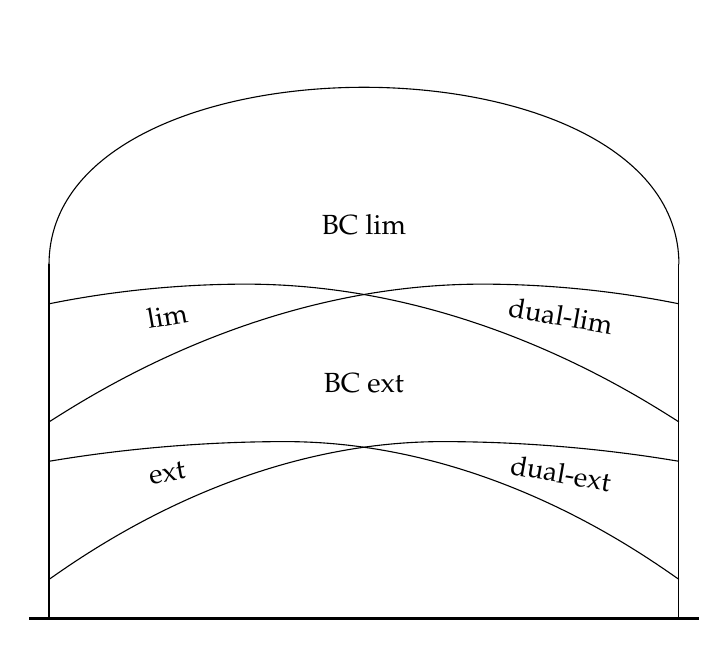
\begin{tikzpicture}
\pgftransformscale{.50}

% http://www.texample.net/tikz/examples/complexity-classes/

%%% HELP LINES - uncomment to design/extend
% \draw[step=1cm,gray,very thin] (-10,0) grid (10,12);
% \node at (0,0) {\textbf{(0,0)}};

%% Horizontal bar
\draw[very thick] (8.5,0) -- (-8.5,0);

% BC lim
\draw (-8,0) -- (-8,9);
\draw (-8,9) .. controls (-8,15) and (8,15) .. (8,9);
\draw (8,0) -- (8,9);
\node at (0,10) {BC lim};

% lim
\draw (-8,8) parabola bend (-3,8.5) (8,5);
\node[rotate=10] at (-5,7.7) {lim};

% dual-lim
\draw (-8,5) parabola bend (3,8.5) (8,8);
\node[rotate=-10] at (5,7.7) {dual-lim};

% BC ext
\node at (0,6) {BC ext};

% ext
\draw (-8,4) parabola bend (-2,4.5) (8,1);
\node[rotate=10] at (-5,3.7) {ext};

% dual-ext
\draw (-8,1) parabola bend (2,4.5) (8,4);
\node[rotate=-10] at (5,3.7) {dual-ext};

\end{tikzpicture}
\end{center}
\end{frame}

\begin{frame}[<+->]{Questions}
\begin{itemize}
\item instead of the class of regular $*$-languages, look at other $*$-language classes, e.g. starfree, $\LT$, $\PT$, or any arbitrary $*$-language class $\Lang$
\item does it result in the same relations as in the diagram? are the enclosures strict?
\end{itemize}
\

My Diplom thesis:
\begin{itemize}
\item Chapter 3: general results on arbitrary $\Lang$, given some introduced properties on $\Lang$
\item Chapter 4: concrete $*$-language classes
\end{itemize}
\end{frame}

\begin{frame}[<+->]{Properties on $\Lang$}
Let $L,A,B \in \Lang$.
\begin{enumerate}
\item \defword{Closure under suffix-independence}: $L \cdot \Sigma^* \in \Lang$
\item \defword{Closure under union, intersection}: $A \cup B \in \Lang$, $A \cap B \in \Lang$
\item \defword{Closure under negation}: $-L \in \Lang$
\item \defword{Closure under change of final states}:
Let $\A_L = (Q,\Sigma,q_0,\delta,F_L)$ be the minimal deterministic automaton for $L$, i.e. with $L^*(\A_L) = L$. Then, for all $F' \subseteq Q$, we have $L^*((Q,\Sigma,q_0,\delta,F')) \in \Lang$.
\item \defword{Closure under alphabet permutation}: For all permutations $\sigma : \Sigma \rightarrow \Sigma$, we have $L_\sigma := \Set{\sigma(w)}{w \in L} \in \Lang$
\end{enumerate}
\end{frame}

\begin{frame}[<+->]{General results}
\begin{itemize}
\item Lemma 3.3: Closure under suffix-independence $\Rightarrow$ \\
$\ext \Lang \subseteq \lim \cap \dlim \Lang$ (but $\not\Leftarrow$)
\item Lemma 3.8: Closure under suffix-independence and negation $\Rightarrow$ \\
$\ext \cup \dext \Lang \subseteq \lim \cap \dlim \Lang$
\end{itemize}

\

Separating language for $\ext \cup \dext \subsetneqq \BC \ext$, $\lim \cup \dlim \subsetneqq \BC \lim$: \\
$\Sigma := \Set{a,b,c}$, $L_a := \Sigma^* a$, $L_b := \Sigma^* b$. \\
$\tilde L_1 := \ext L_a \cap -\ext L_b$, $\tilde L_2 := \lim L_a \cap -\lim L_b$. \\
$\tilde L_1 \not\in \ext \cup \dext \Lang$ but $\tilde L_1 \in \BC \ext \Lang$. \\
$\tilde L_2 \not\in \lim \cup \dlim \Lang$ but $\tilde L_2 \in \BC \lim \Lang$.

More general:
\end{frame}

\begin{frame}[<+->]{General results}
\textbf{Definition 3.12.} A language $L \subseteq \Sigma^* \cup \Sigma^\omega$ is called \defword{$M$-invariant} for $M \subseteq\Sigma$ iff for all $w \in \Sigma^* \cup \Sigma^\omega$,
\[ w \in L \ \ \ \Leftrightarrow \ \ \  w |_M \in L , \]
where $w|_M$ is the word $w$ with all letters from $M$ removed.

There is always exactly one \defword{maximum invariant alphabet set $M_m \subseteq \Sigma$ of $L$} such that $L$ is $M_m$-invariant. Then call $\Sigma-M_m$ the \defword{non-invariant alphabet set of $L$}.

\

\textbf{Theorem 3.15.} Let $\Lang$ be closed under negation and under alphabet permutation. Let $\Set{a,b,c} \subseteq \Sigma$. Let there be $L_a \in \Lang$. Let $\Set{a}$ be the \emph{non-invariant alphabet set of $L_a$} and let $L_a$ be \emph{$\Set{b,c}$-invariant}. Then
\[ \ext L_a \not\in \dext \Langreg \ \ \ \Rightarrow \ \ \ \ext \cup \dext \Lang \subsetneqq \BC \ext \Lang \]
and
\[ \lim L_a \not\in \dlim \Langreg \ \ \ \Rightarrow \ \ \ \lim \cup \dlim \Lang \subsetneqq \BC \lim \Lang . \]
\end{frame}

\begin{frame}[<+->]{General results}
\begin{itemize}
\item \textbf{Theorem 3.19.} (Staiger-Wagner 1) $\Lang$ closed under change of final states. Then
\[ \lim \cap \dlim \Lang \subseteq \BC \ext \Lang . \]
\item \textbf{Theorem 3.20.} (Staiger-Wagner 2) $\Lang$ closed under suffix-independence, negation, union and change of final states. Then
\[ \BC \ext \Lang \subseteq \lim \cap \dlim \Lang . \]
\item \textbf{Theorem 3.22.} $\Lang$ closed under suffix-independence, negation, union, change of final states and alphabet permutation.
Then we have
\begin{align*}
& \ext \cap \dext \Lang \stackrel{(1.)}\subseteq
\ext \cup \dext \Lang \stackrel{(2.)}\subseteq
\BC \ext \Lang \stackrel{(3.)}= \\
& \lim \cap \dlim \Lang \stackrel{(4.)}\subseteq
\lim \cup \dlim \Lang \stackrel{(5.)}\subseteq
\BC \lim \Lang .
\end{align*}
With $\Lang$-$\ext$-$\dext$-separating language $L_a$, the inclusions in (1) and (2) are strict.
With $\Lang$-$\lim$-$\dlim$-separating language $L'_a$, the inclusions in (4) and (5) are strict.\end{itemize}
\end{frame}

\begin{frame}[<+->]{General results: Kleene closure}
\[ \Kleene(\Lang) := \Set{ \bigcup_{i=1}^n U_i \cdot V_i^\omega}{U_i, V_i \subseteq \Sigma^*, U_i \cdot V_i^* \in \Lang, n \in \N_0} \]

\begin{itemize}
\item \textbf{Lemma 3.24.} $\Lang$ closed under change of final states for all deterministic simplified automata. Then
\[ \Kleene \Lang \subseteq \BC \lim \Lang . \]
(The closure of final states here is stronger.) (The idea in the proof can probably be generalized into a general non-deterministic Büchi to deterministic Muller automaton conversion.)
\item \textbf{Lemma 3.25.} $\Lang$ closed under change of final states. Then
\[ \lim \Lang \subseteq \Kleene \Lang . \]
\end{itemize}
\end{frame}

\begin{frame}[<+->]{Concrete results}
\begin{enumerate}
\item $ \BC \ext \Lang^* (\PT) = \BC \lim \Lang^* (\PT) $
\item $ \Lang^\omega (\mathrm{FO[+1]}) = \BC \ext \Lang^*(\mathrm{FO[+1]}) $
\item $ \Lang^\omega (\mathrm{FO[<]}) = \BC \lim \Lang^*(\mathrm{FO[<]}) $
\item $ \BC \ext \Lang^*( \mathrm{FO[<]} ) \subsetneqq \BC \lim \Lang^* ( \mathrm{FO[<]} )  $
\item $ \BC \ext \Lang^* (\LT) \subsetneqq \BC \lim \Lang^*(\LT) $
\item $ \BC \ext \Lang^* (\posPT) = \BC \lim \Lang^* (\posPT) $
\item $ \BC \ext \Lang^*(\posPT) = \BC \ext \Lang^* (\PT) $
\end{enumerate}
\end{frame}

\end{document}
